
% !TEX encoding = UTF-8 Unicode 
% !TEX root = FieldGuide.tex

\Sec[Gen. Beta Prime Distribution] {Generalized Beta Prime Distribution}
\label{sec:GenBetaPrime}
\phantomsection
\addcontentsline{toc}{subsection}{~~~~~~~~~~~~Generalized beta prime} 
The {\bf Generalized beta prime} (Feller-Pareto, beta-log-logistic, generalized\linebreak gamma ratio, Majumder-Chakravart, generalized beta type II, generalized Feller-Pareto)  distribution~\cite{Feller1971, McDonald1984, Tahmasebi2010} is a five parameter,  continuous, univariate, unimodal probability density, with semi-infinite support. The functional form in the most straightforward parameterization is
\begin{align}
\label{GenBetaPrime}
\opr{GenBetaPrime}&(x\given a, s, \alpha,\gamma,\beta) \\
& =
 \frac{1}{B(\alpha, \gamma)} \left|\frac{\beta}{s}\right|
\left(\frac{x-a}{s}\right)^{\alpha\beta -1} \left(1+ \left(\frac{x-a}{s}\right)^\beta \right)^{-\alpha-\gamma }
\notag
\checked
\\ & \quad a,\ s,\ \alpha,\ \gamma,\ \beta \text{ in } \mathbb{R},\quad  \alpha,\ \gamma >0
\notag
\end{align}
The five real parameters of the generalized beta prime distribution consist of a location parameter~$a$, 
scale parameter~$s$, two shape parameters,~$\alpha$ and~$\gamma$, and the Weibull power parameter $\beta$. The shape parameters, $\alpha$ and $\gamma$, are positive.


The generalized beta prime arises as the Weibull transform of the standard beta prime distribution \eqref{StdBetaPrime}, and as order statistics of the log-logistic distribution. The Amoroso distribution is a limiting form, and a variety of other distributions occur as special cases. (See Table~\ref{GenBetaPrimeTable}).  These distributions are most often encountered as parametric models for survival statistics developed by  economists and actuaries.




\SSec{Special cases}



\dist {Transformed beta} distribution~\cite{McDonald1984,Klugman2012}:
\begin{align}
\label{TransformedBeta}
\opr{TransformedBeta}&(x\given s, \alpha,\gamma,\beta) 
\\ \notag & =
 \frac{1}{B(\alpha, \gamma)} \left|\frac{\beta}{s}\right|
\left(\frac{x}{s}\right)^{\alpha\beta -1} \left(1+ \left(\frac{x}{s}\right)^\beta \right)^{-\alpha-\gamma }
\checked
\\ \notag &= \opr{GenBetaPrime}(x\given 0, s, \alpha,\gamma,\beta) 
\checked
\end{align}
A generalized beta prime distribution without a location parameter, $a=0$.


\dist{Burr}  (Burr type XII, Pareto type IV, beta-P, Singh-Maddala, generalized log-logistic, exponential-gamma,Weibull-gamma) 
%q-exponential\sscite{Nadarajah2006}) %This dosn't compute.
distribution~\cite{Burr1942,Tadikamalla1980, Kleiber2003}:
\begin{align}
\label{Burr}
\opr{Burr}(x\given a, s, \gamma,\beta) 
&=  
 \frac{\beta \gamma}{|s|} \left(\frac{x-a}{s}\right)^{\beta-1}  \left(1+\left(\frac{x-a}{s}\right)^\beta\right)^{-\gamma-1} 
 \checked
\\ & = \opr{GenBetaPrime}(x\given a, s, 1,\gamma,\beta) \notag   \checked
\end{align}
Most commonly encountered as a model of income distribution.



\begin{table*}[tp]
%\addcontentsline{toc}{subsection}{Beta prime} 
\begin{center}
\caption[Generalized beta prime distribution -- Special cases]{Special cases of generalized beta prime}
\label{GenBetaPrimeTable}
~\\
{\renewcommand{\arraystretch}{1.25} 
\begin{tabular}{llccccc}
\eqref{GenBetaPrime}  & generalized beta prime & $a$ & $s$ & $\alpha$  &  $\gamma$ & ${\beta}$  \\
\hline
\eqref{Burr} & Burr 	        			&  .  &  .  &  1  &  .    &    .     \\
\eqref{Dagum} & Dagum			&  0  &  1 &  .  &  1   &    .     \\
\eqref{Paralogistic} & paralogistic			&  0 &  1  &  1  &  $\beta$    &    .     \\
\eqref{InvParalogistic} & inverse paralogistic	&  0 &  1  &   $\beta$& 1    &    .     \\
\eqref{LogLogistic} & log-logistic			&  0  &  . &  1  &  1  &    .     \\
\eqref{GenBetaPrime} & transformed beta			&  0  &  . &  .  &  .  &    .     \\
\eqref{HalfGenPearsonVII} & half gen. Pearson VII 		&  .  &  . &  $\tfrac{1}{\beta}$  &  $m$-$\tfrac{1}{\beta}$  &    .     \\
\eqref{BetaPrime} & beta prime		& . & . & . & . & 1  \\
%\eqref{Pareto} & Pareto 				&  $s$  &  . &  1  &  .   &    1     \\
\eqref{Lomax} & Lomax 				&  .  &  . &  1  &  .   &    1     \\
\eqref{InvLomax} & inverse Lomax 				&  .  &  . &  .  &  1   &    1     \\
\eqref{StdBetaPrime} & std. beta prime		& 0 & 1 & . & . & 1  \\
\eqref{F} & F	&  0 &  $\tfrac{k_2}{k_1}$ & $\tfrac{k_1}{2}$ & $\tfrac{k_2}{2}$   &    1     \\
\eqref{UniPrime} & uniform-prime	& . & . & 1 & 1 & 1  \\
\eqref{ExpRatio} & exponential ratio		& 0 & . & 1 & 1 & 1  \\
\eqref{HalfPearsonVII} & half-Pearson  VII	&  . &  .  &   $\tfrac{1}{2}$ & .   &    2     \\
\eqref{HalfCauchy} & half-Cauchy	&  . &  . & $\tfrac{1}{2}$ & $\tfrac{1}{2}$   &    2     \\
%\eqref{Moffat} & Moffat	&  0 &  . & 1 & .   &    2     \\
%\\
%& \underline{Limits}  \\
%\eqref{Amoroso} & Amoroso	~~~ $\lim_{\gamma\rightarrow+\infty}$		& . & $\theta \gamma^{\frac{1}{\beta}}$& . & $\gamma$ & .      \\
%\eqref{BetaLogistic} & beta-logistic	~~~~~$\lim_{\beta\rightarrow-\infty}$		& ${\pLoc\text{-}\beta\pScale}$ & $\beta\pScale$ & . & . &$\beta$      % Need minus sign (in limit?) else alpha and gamma flip
\end{tabular} 
}
\end{center}
\end{table*}


% !TEX encoding = UTF-8 Unicode 
% !TEX root = FieldGuide.tex

\begin{table*}[p]
\caption[Generalized beta prime distribution -- Properties]{Properties of the generalized beta prime distribution}
\begin{align*}
 \text{\hyperref[PropertiesSec]{Properties}}  \quad& \\
\text{notation} \quad & \text{GenBetaPrime}(x\given a, s, \alpha,\gamma,\beta)   \checked
\\
\text{PDF}\quad &    \frac{1}{B(\alpha, \gamma)} \Left|\frac{\beta}{s}\Right|	
\Left(\frac{x-a}{s}\Right)^{\alpha\beta -1} \Left(1+ \Left(\frac{x-a}{s}\Right)^\beta \Right)^{-\alpha-\gamma } \checked
\hspace{-30em}
\\
\text{CDF / CCDF} \quad  &  
\frac{B\big(\alpha, \gamma; (1+(\tfrac{x-a}{s})^{-\beta})^{-1} \big) }{B(\alpha,\gamma)} \checked
\hspace{-7em}
& \tfrac{\beta}{s} >0 \,\big/ \, \tfrac{\beta}{s} <0
\\ 
& \quad = I\Left(  \alpha,\gamma; (1+(\tfrac{x-a}{s})^{-\beta})^{-1} \Right)  \checked
% See McDonald1984, table 3.1 GB2. Expresses incomplete beta function as hypergeometric function.
\\
\text{parameters}\quad &   a,\ s,\ \alpha,\ \gamma,\ \beta \text{ in } \Real \checked 
\\ & \alpha>0, \gamma>0	\checked
\\
\text{support} \quad &    x \geq a &  s > 0 										
\\
&  x\leq a  &  s < 0 
\\
%\text{median} \quad  &  \cdots
%\\
% \text{mode} \quad  & \cdots
% \\
\text{mean} \quad  &   a+\frac{s B(\alpha+\tfrac{1}{\beta},\gamma- \tfrac{1}{\beta}) }{B(\alpha,\gamma)} 
\checked &   -\alpha< \tfrac{1}{\beta} <\gamma \checked
% % See McDonald1984, table 3.1 GB2
\\
\text{variance} \quad  &s^2\Left[\frac{ B(\alpha+\tfrac{2}{\beta},\gamma- \tfrac{2}{\beta}) }{B(\alpha,\gamma)} -  \Left(\frac{ B(\alpha+\tfrac{1}{\beta},\gamma- \tfrac{1}{\beta}) }{B(\alpha,\gamma)}\Right)^2 \Right]  \hspace{-15em}
& -\alpha< \tfrac{2}{\beta} <\gamma \checked
\\
\text{skew} \quad  &  \text{not simple}
\\
\text{kurtosis} \quad  &  \text{not simple}
%\\
%\text{entropy} \quad  &   \ln \frac{1}{B(\alpha, \gamma)} \Left|\frac{\beta}{s}\Right|
%  +(\tfrac{1}{\beta}-\alpha) \big[ \psi(\alpha) - \psi(\gamma)\big]
%  \hspace{-7em} 
%  \\
%& \quad +(\alpha+\gamma) \big[ \psi(\alpha+\gamma) - \psi(\gamma)\big] \checked & \text{\cite[Eq.~(15)]{Tahmasebi2010}} % Not correct?
\\
% \text{MGF} \quad  &  \cdots
% \\
% \text{CF} \quad  &  \cdots
% \\
E[ X^h]  \quad & \frac{|s|^h B(\alpha+\tfrac{h}{\beta},\gamma- \tfrac{h}{\beta}) }{B(\alpha,\gamma)} 
& \!\!a=0,\  -\alpha< \tfrac{h}{\beta} <\gamma \quad   \text{\cite{McDonald1984}} \checked
\end{align*}
\end{table*}






\dist{Dagum} (Inverse Burr, Burr type III, Dagum type I,  beta-kappa, beta-k, Mielke) distribution~\cite{Burr1942, Dagum1977, Tadikamalla1980}:
\begin{align}
\label{Dagum}
\opr{Dagum}(x\given  \gamma,\beta) 
%&= \gamma \beta \frac{x^{\gamma\beta-1}}{ (1+x^\beta)^{\gamma +1} }  \\
&=  \frac{\beta \gamma}{|s|} \left(\frac{x-a}{s}\right)^{\gamma \beta-1}  \left(1+\left(\frac{x-a}{s}\right)^\beta\right)^{-\gamma-1} 
\checked
%\\ \notag &= \opr{Burr}(x\given a,s,  \gamma,-\beta) \checked % Burr restricted to positive beta
\\ \notag &= \opr{GenBetaPrime}(x\given a, s, 1, \gamma,-\beta) \checked
\\ \notag &= \opr{GenBetaPrime}(x\given a, s, \gamma,1,+\beta) \checked
\end{align}

\dist{Paralogistic} distribution~\cite{Kleiber2003}:
\begin{align}
\label{Paralogistic}
\opr{Paralogistic}(x\given a, s, \beta) &= \frac{\beta^2}{|s|} \frac{ \left(\frac{x-a}{s}\right)^{\beta-1}}{ (1+ \left(\frac{x-a}{s}\right)^\beta)^{\beta+1} } \checked
\\ \notag &= \opr{GenBetaPrime}(x\given a, s, 1,\beta,\beta) 
\end{align}


\dist{Inverse paralogistic} distribution~\cite{Klugman2012}:
\begin{align}
\label{InvParalogistic}
\opr{InvParalogistic}(x\given a,s,\beta) &= \frac{\beta^2}{|s|}  \frac{ \left(\frac{x-a}{s}\right)^{\beta^2-1}}{ (1+ \left(\frac{x-a}{s}\right)^\beta)^{\beta+1} } \checked
\\ \notag &= \opr{GenBetaPrime}(x\given a, s, \beta,1,\beta) \checked
\end{align}





\dist{Log-logistic} (Fisk, Weibull-exponential, Pareto type III, power prime) distribution~\cite{Shah1963, Johnson1995}:
\begin{align}
\label{LogLogistic}
\opr{LogLogistic}(x\given a,s,\beta) &=\left|\frac{\beta}{s}\right| \frac{\left(\frac{x-a}{s}\right)^{\beta-1}}{ \left(1+\left(\frac{x-a}{s}\right)^{\beta}\right)^{2} } \checked
\\ \notag &= \opr{Burr}(x\given a, s, 1,\beta) \checked
\\ \notag &= \opr{GenBetaPrime}(x\given 0, s, 1,1,\beta) \checked
\end{align}
Used as a parametric model for survival analysis and, in economics, as a model for the distribution of wealth or income.
The logistic and log-logistic distributions are related by an exponential transform. 
\[
\opr{LogLogistic}(0,s,\beta) &\sim  \exp\bigl(-\opr{Logistic}(-\ln s,\sfrac{1}{\beta})\bigr) 
\checked
\notag
\]

\begin{figure}[t]
\begin{center}
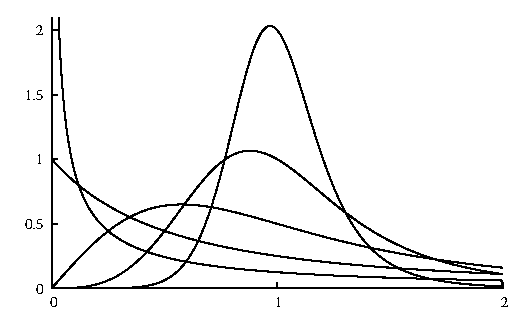
\includegraphics[width=\textwidth]{pdfLogLogistic}
\end{center}
\caption[Log-logistic distributions]{Log-logistic distributions, $\opr{LogLogistic}(x\given 0,1,\beta)$.}
\end{figure}




\dist{Half-Pearson VII} (half-t) distribution~\cite{Gelman2006}: 
\begin{align}
\label{HalfPearsonVII}
 \opr{HalfPearsonVII}&(x\given a, s, m)  \\
\notag &=
 \frac{1}{B(\tfrac{1}{2},m-\tfrac{1}{2})} \frac{2}{|s|}
 \left(1+ \left(\frac{x-a}{s}\right)^2 \right)^{-m} \checked
\\ \notag & =  \opr{GenBetaPrime}(x\given a, s, \tfrac{1}{2},m-\tfrac{1}{2}, 2) \checked
\end{align}
The Pearson type VII \eqref{PearsonVII} distribution truncated at the center of symmetry. Investigated as a prior for variance parameters in hierarchal models~\cite{Gelman2006}.



\dist{Half-Cauchy} distribution~\cite{Gelman2006}: 
\begin{align}
\label{HalfCauchy}
\opr{HalfCauchy}(x\given a, s)  &=
 \frac{2}{\pi |s|}
 \left(1+ \left(\frac{x-a}{s}\right)^2 \right)^{-1}
 \checked
 \\ \notag & =  \opr{HalfPearsonVII}(x\given a, s, 1) \checked
\\ \notag & =  \opr{GenBetaPrime}(x\given a, s, \tfrac{1}{2},\tfrac{1}{2}, 2)  
\checked
\end{align} 
A notable subclass of the Half-Pearson type VII, the Cauchy distribution \eqref{Cauchy} truncated at the center of symmetry.


\dist{Half generalized Pearson VII} distribution~\cite{\self}: 
\begin{align}
\label{HalfGenPearsonVII}
\opr{HalfGenPearsonVII}&(x\given a,s, m,\beta)  
\\ \notag = & \frac{\beta}{ |s| B(m-\frac{1}{\beta}, \frac{1}{\beta} )} \left( 1 +\left( \frac{x-a}{s}\right)^{\beta} \right)^{-m} 
\checked
\\ \notag & =  \opr{GenBetaPrime}(x\given a, s, \tfrac{1}{\beta},m-\tfrac{1}{\beta}, \beta) 
\checked
%\\ \notag & x, a,s, m,\beta \text{ in } {\mathbb R} \\
%&  \tfrac{x-a}{s}>0,\  \beta>0,\ m>0,\ \beta m >1
%\notag
\end{align}
One half of a Generalized Pearson VII distribution~\eqref{GenPearsonVII}. 
Special cases include half Pearson VII \eqref{HalfPearsonVII}, half Cauchy \eqref{HalfCauchy}, {\bf half Laha} (See \eqref{Laha}),  and uniform prime \eqref{UniPrime} distributions. 
\begin{align*}
\opr{HalfGenPearsonVII}(x\given a,s, m,2) &= \opr{HalfPearsonVII}(x\given a,s,m) \checked \\
\opr{HalfGenPearsonVII}(x\given a,s, 1,2) &= \opr{HalfCauchy}(x\given a,s) \checked \\
\opr{HalfGenPearsonVII}(x\given a,s, 1,4) &= \oprr{HalfLaha}{Laha}(x\given a,s) \checked \\
\opr{HalfGenPearsonVII}(x\given a,s, 2,1) &= \opr{UniPrime}(x\given a,s)  \checked 
\end{align*}
The half exponential power \eqref{HalfExpPower} distribution occurs in the large $m$ limit.
\begin{align*}
\lim_{m\rightarrow\infty} \opr{HalfGenPearsonVII}&(x\given a,\theta m^{\sfrac{1}{\beta}}, m,\beta) 
 = \opr{HalfExpPower}(x\given a,\theta,\beta) \checked
\end{align*}
\phantomsection
\addcontentsline{toc}{subsection}{~~~~~~~~~~~~Half Laha}



% ====================================================================
\SSec{Interrelations}


Negating the Weibull parameter of the generalized beta prime distribution is equivalent to exchanging the shape parameters  $\alpha$ and $\gamma$.
\begin{align*}
\opr{GenBetaPrime}&(x\given a, s, \alpha,\gamma,\beta)  = \opr{GenBetaPrime}(x\given a, s,\gamma, \alpha,-\beta) \checked
\end{align*}

The distribution is related to ratios of gamma distributions.
\[
\opr{GenBetaPrime}(a,s,\alpha,\gamma,\beta) \sim a+ s\left( \frac{\opr{StdGamma}_1(\alpha)}{\opr{StdGamma}_2(\gamma) } \right)^{\tfrac{1}{\beta}} \checked
\]

Limit of the generalized beta prime distribution include the Amoroso \eqref{Amoroso}~\cite{McDonald1984} and beta-logistic \eqref{BetaLogistic} distributions.
\begin{align*}
\lim_{\gamma\rightarrow\infty} \opr{GenBetaPrime}(x\given a, \theta \gamma^{\frac{1}{\beta}} ,\alpha, \gamma, \beta )  
%\\ 
& = \opr{Amoroso}(x\given a,\theta,\alpha, \beta) \checked \\
\lim_{\beta\rightarrow\infty}  \opr{GenBetaPrime}(x\given  \pLoc+\beta\pScale, -\beta \pScale, \alpha, \gamma, \beta)  
 %\\
 & = \opr{BetaLogistic}(x\given \pLoc,\pScale, \gamma, \alpha) \checked
\end{align*}
Therefore, the generalized beta prime also indirectly limits to the normal \eqref{Normal}, log-normal \eqref{LogNormal}, gamma-exponential \eqref{GammaExp}, Laplace \eqref{Laplace} and power-function \eqref{PowerFn} distributions, among others.

Generalized beta prime describes the order statistics \secref{OrderStatistic} of the log-logistic distribution \eqref{LogLogistic}). 
\begin{align*}
 \opr{OrderStatistic}_{\opr{LogLogistic}(a,s,\beta)}(x \given \gamma, \alpha ) & =  \opr{GenBetaPrime}(x\given a, s, \alpha, \gamma, \beta)  \checked
\end{align*}


Despite occasional claims to the contrary,%~\cite{???,???,???}, 
the log-Cauchy distribution is not a special case of the generalized beta prime distribution (generalized beta prime is mono-modal, log-Cauchy is not).





% =================================================================================
